\documentclass[12pt]{article}
\usepackage{fullpage,graphicx,psfrag,amsmath,amsfonts,verbatim,booktabs}
\usepackage{colortbl,xcolor}

\usepackage[small,bf]{caption}
\usepackage{algorithmicx,algpseudocode}
\usepackage{url,algorithm}
\newtheorem{lem}{Lemma}
\usepackage[toc,page]{appendix}
\bibliographystyle{alpha}
\input defs.tex

\usepackage{hyperref}
\hypersetup{
    colorlinks=true,%
    citecolor=blue,%
    filecolor=blue,%
    linkcolor=blue,%
    urlcolor=blue
}
\pagestyle{plain}

\title{Generalized Blind Deconvolution}

\author{Qingyun Sun
\and Stephen Boyd}

\begin{document}
\maketitle
% \begin{abstract}
% \end{abstract}
\section{Introduction}
Blind Deconvolution is the problem of recovering a kernel and a signal from their convolution. This is an ubiquitous problem in fields including signal processing, machine learning, communication, seismology, computer vision, microscopy, neural science. 

\section{Generalized blind deconvolution}
\subsection{Problem formulation}
Consider that we have an observation vector $y\in\reals^n$, and we want to look for a filter $w\in \mathcal W\subset \reals^n$ such that the circular convolution $w*y\in\reals^n$ is close to a signal $x\in \mathcal X\subset \reals^n$ that is simple under certain measure, for example, sparsity. 
 More precisely, we can write 
\[
w*y \approx x + \epsilon,
\]
where $\epsilon$ is the noise or error of approximation. 

We need to normalize $w$, otherwise $w$ equals zero will result in a trivial signal. We impose that $\mathcal W$ does not contain zero, and if $w \in \mathcal W$, then $cw\in \mathcal W$ imply $c=\pm 1$.  

Mathematically, given an observation $y\in \reals^n$, we want to find a kernel $w \in \mathcal W,$ and a signal $x\in \mathcal X$ such that 
\BEQ
\label{gcbd}
\begin{array}{ll}
\mbox{minimize}   & l(x-y*w)+r(x)+ s(w)\\
\mbox{subject to} &  w \in \mathcal W, \qquad x \in \mathcal X
\end{array}
\EEQ
with variable $w,x$ in subsets $\mathcal W, \mathcal X$ of $\reals^n$. 
 $l$ is the loss function that measure how well the approximation is. $r$ is the regularizer on signal,  $s$ is the regularizer on kernel. 
 
 We can incorporate the indicator functions of the constraint in the regularizers, and define  $R = r + I_{ \mathcal X},$
 $S = s +I_{ \mathcal W}$. Then the problem becomes
 \BEQ
\label{gcbd2}
\begin{array}{ll}
\mbox{minimize}   & l(x-y*w)+R(x)+ S(w)
\end{array}
\EEQ
%  \begin{eqnarray*}
% \underset{w, x }{\mbox{minimize}}& L(x,y*w)+R_1(x)+ R_2(w),\\
% \mbox{subject to}& e^T w =1.
%  \end{eqnarray*}
%  Here $e\in \mathbb{R}^k$ is a unit vector, and the constraint $e^T w =1$ is a normalization of $w$.  
 

 This is a discriminative model approach of blind deconvolution. The advantage of this problem is that it is a convex problem if $l$, $R$ and $S$ are convex functions.
 
Even when one of them is not convex, as long as the proximal operator is computable, we can still use ADMM based method to approximately solve the problem.
\subsection{Examples}
Now we enumerate a few different choices for $l, r, s, \mathcal X, \mathcal W$.
\paragraph{Choice of $l$.}
For $l$, the most common choice is $l(u) = \|u\|_2^2$. Other choices are $l(u) =\|u\|_1$ or Huber function. In general, $l$ is the negative log-likelihood of the noise distribution.
\paragraph{Choice of $r$ and $s$. }
$r$ is the simplicity measure of the signal. One family of common examples are $r(x) = \|x\|_1, \|Dx\|_1$ and $L_1$ norm for higher order derivative. We can also replace $L_1$ norm with Huber function and $\|x\|_2^2$. Another important family of choices are the higher other cumulants, which is to encourage the non-Gaussian property of the signal if we treat it as a sample of stochastic process. 

For $s$, we can still choose the simplicity measure as discussed in $r$. We can also choose $s$ to be simplicity measure on Fourier transform of the kernel. If we use Bayesian method and have a prior on the kernel, we can choose $s$ as the logarithm of the prior distribution. 

\paragraph{Choice of $\mathcal X$ and $\mathcal W$. }
For $\mathcal X$, one natural example is that the sparsity level of $x$ is below threshold $k$. It is a non-convex constraint but we can compute the projection on this constraint set by hard-thresholding. 

For $\mathcal W$, we must fix the scale of $w$, or at least low-bound $w$ away from $zero$ to get a non-trivial solution.  As discussed before, a subset $\mathcal W$ fixes scale if it does not contain zero and if $w \in \mathcal W$, then $cw\in \mathcal W$ imply $c=\pm 1$.  
One natural choice of $\mathcal W$ is to fix some coordinate of $w$, for example, $w_1=1$. In general, we can fix a nonzero vector $e$, and fix $e^T w =1$. Another choice is $\|w\|_2=1$, which is non-convex, but the projection is easy to compute. Besides the equality constraint that fixes scale, we can also constraint the length of $w$, for example, we can impose that only the first $k$ coordinates of $w$ can be non-zero. 
\subsection{Optimization method}
 To solve this problem, we can rewrite the problem as
\BEQ
\begin{array}{ll}
\mbox{minimize}   & l(x-z)+R(\tilde{x})+ S(\tilde{w}) \\
\mbox{subject to}  & z = y*w,\\
& w = \tilde{w},\\
& x = \tilde{x},
\end{array}
\EEQ
with variables $w, \tilde{w},x, \tilde{x}, z\in \reals^n$.

 Then we can use alternating direction method of multiplier to solve this problem when the problem is convex. 
  The augmented Lagrangian for this problem is 
\begin{eqnarray*}
 \mathcal{L}_{s_1, s_2,s_3}(w, \tilde{w},x, \tilde{x}, z, u_1, u_2, u_3)&=&l(x-z)+R(\tilde{x})+ S(\tilde{w})+
 \frac{s_1}{2} \| z -y*w -u_1\|^2 \\
 & & + \frac{s_2}{2} \| x- \tilde{x}-u_2\|^2+
 \frac{s_3}{2} \| w- \tilde{w}-u_3\|^2,
\end{eqnarray*}
where $u_1, u_2, u_3$ are the scaled dual variables, $s_1, s_2,s_3$ are positive.

If we assume $l,R,S$ are all convex functions, we can define a new variable $v := (w, \tilde{w},x, \tilde{x}, z)$, the objective function $f(v) = f(w, \tilde{w},x, \tilde{x}, z):=l(x-z)+R(\tilde{x})+ S(\tilde{w})$, and write the linear constraints as $v\in C$. Then the problem is
  \BEQ
\label{gcbd3}
\begin{array}{ll}
\mbox{minimize}   & f(v) \\
\mbox{subject to} & v\in C,
\end{array}
\EEQ
with variable $v$.
Then it is a convex problem with linear constraint, we can apply the standard ADMM algorithm from chapter $5$ of \cite{boyd2011distributed}. 
\begin{equation}
\label{scaled_admm}
  \begin{split}
&v^{k+1/2} := \mathrm{prox}_{f}(v^{k}-\tilde{v}^{k})\\
&v^{k+1} :=  \Pi\left(v^{k+1/2}+\tilde{v}^k\right)\\
&\tilde{v}^{k+1} :=  \tilde{v}^k + v^{k+1/2} - v^k.
\end{split}
\end{equation}

The variable $k$ is the iteration counter, $v^{k+1/2}$ and $v^{k}$  are primal
variables, $\tilde{v}^k$ are scaled dual variables.
\[
  \mathrm{prox}_{f}(v) = \argmin_{v'}\Big(f(v') + (\rho/2) \vnorm{v' - v}_2^2\Big)
\]
is the proximal operator of $f$,
and $\rho>0$ is the proximal parameter. To calculate $\mathrm{prox}_{f}$, we only need to calculate the proximal operators $\mathrm{prox}_{l},\mathrm{prox}_{R},\mathrm{prox}_{S}$.
$\Pi$ denotes the (Euclidean)
projection onto the graph define by the linear constraint $C$, it can be explicitly expressed as the projections on the three equations $z = y*w, w = \tilde{w}, x = \tilde{x}$. The last two projections are averaging of $w, \tilde{w}$ and $x, \tilde{x}$. 
The first projection is a projection on the graph form  $z = y*w$, we can apply the graph projection splitting algorithm \cite{fougner2015parameter} to this problem. One advantage of convolution is that we can leverage the convolution theorem, and compute the projection of $(z,w)$ onto $z = y*w$ using Fourier transform, $\hat z =\hat y  \circ \hat w$, where $ \circ$ is the Hadamard product.  
This update can be computed on each coordinate
\begin{eqnarray*}
    \hat z^{t} &=& \mathcal{F}  z^{t},\\
    \hat w^{t} &=& \mathcal{F}  w^{t}, \\
 (\hat z^{t+1}_i, \hat w^{t+1}_i) &=& \Pi_{\hat y^{t+1}_i}(\hat z^{t+1}_i, \hat w^{t+1}_i).
\end{eqnarray*} 
  
 Here the projection  is given by
\begin{eqnarray*}
 \Pi_{\hat y_i}(\hat z_i, \hat w_i)= ((\hat z_i+ \hat y_i \hat w_i)/(1+\hat y_i^2), \hat y_i(\hat z_i+ \hat y_i \hat w_i)/(1+\hat y_i^2)).
  \end{eqnarray*} 
 Using Fast Fourier transform, we can compute this update in $O(n\log n)$, therefore, the method is suited for large scale problem. 
 After the coordinate-wise projection, we apply inverse Fourier transform to get 
 $z^{t+1}, w^{t+1}$.

\subsection{Numerical example: Sparse blind deconvolution}
 As a primary example of the general framework, we study sparse blind deconvolution problem.  
Assume that we observe $y\in \reals^n$ from the circular convolution of $w$ and $x$, namely,  $y = k*x$, where the signal $x\in \reals^n$ is I.I.D. series sampled from a random variable $X$ with probability $1-p$ to be zero, and probability $p$ to be sampled from a standard Gaussian random variable, and the kernel $k\in \reals^n$ has an inverse $w\in \mathcal W_m \subset \reals^n$ so that $w*k = e_1$, where $e_1=(1,0,\ldots, 0)\in \reals^n$. 
$\mathcal W_m$ is the embedding of $\reals^m$ to the first $m$ coordiantes of $\reals^n$, it contains all the kernels zero-padded from length $m$, and $\mathcal X = \{x\in \reals^n| x_1=1\}$, namely the first coordinate of $x$ is fixed as $1$.
We choose $r(x) = \|x\|_1$ as a convex relaxation of the sparsity measure.  $l$ is the indicator function $I_{x=y*w}$ since the observation is noiseless in this synthetic model. We choose $s=0$ since there is not additional information on the kernel. Therefore, we have the following convex optimization problem:
\BEQ
\label{sbd}
\begin{array}{ll}
\mbox{minimize}   & \|x\|_1\\
\mbox{subject to} &  x=y*w, \quad x_1 =1, \quad w \in \mathcal W_m,
\end{array}
\EEQ
with variable $w\in \mathcal W_m, x\in \reals^n$. 

In the following numerical experiments, we choose the signal length $n=500$, the kernel length $m= 80$, $x$ I.I.D. sampled from product of Bernoulli and normal with sparsity level $0.2$, $w$ I.I.D. sampled from standard normal. We run the above algorithm and We can see that the algorithm can perfectly recover the ground truth signal and kernel.
 
\begin{figure}
  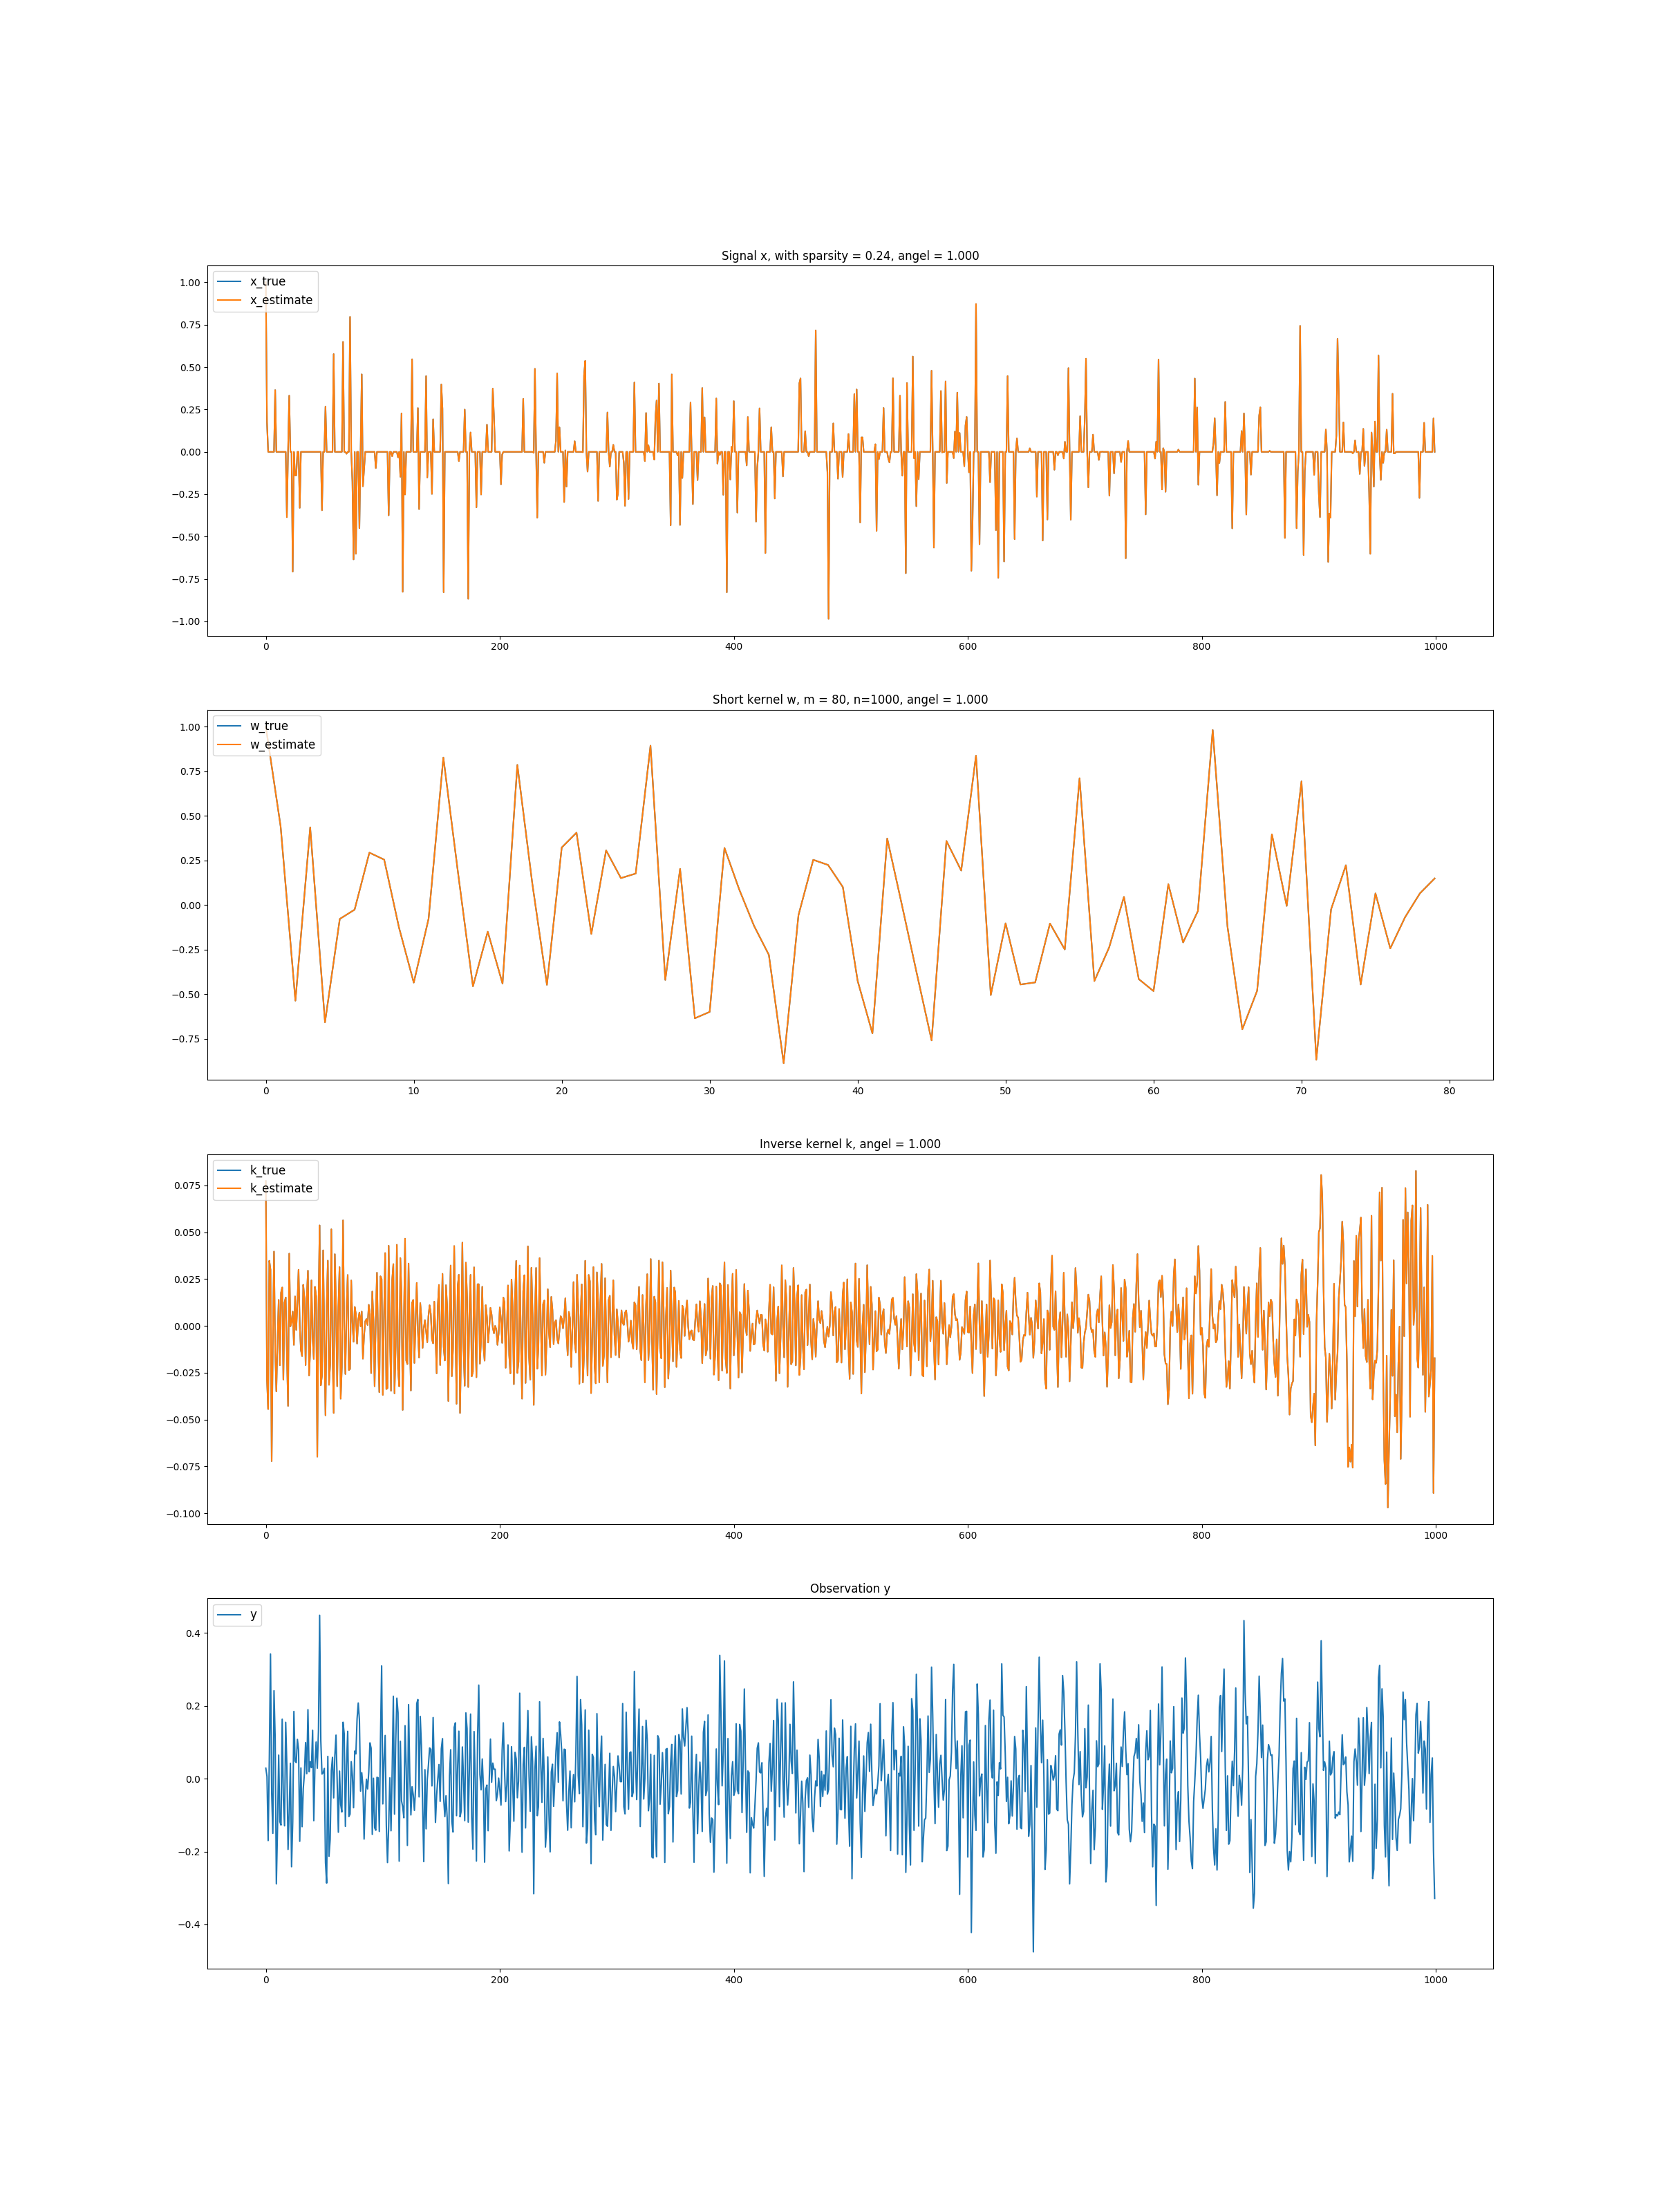
\includegraphics[width=17cm,keepaspectratio]{fig5/bShort_lenKnown_xSparse_w_Gaus_Ano_n1000_k80_p0_24_sigma0_00.png}
\end{figure}
 
\section{Extensions and connections}
\subsection{Generative blind deconvolution }
Consider that we have an observation vector $y\in \reals^n$, and we assume that $y$ is generated by the following model,
\[
y=x*k + e,
\]
where $x\in \mathcal X$ is a signal and $k\in \mathcal K$ is a filter, $e$ is the error of the convolutional approximation. As before, we need to normalize $k$ in the definition of $\mathcal K$ to fix the scale.

Then our optimization problem is
\BEQ
\label{ncbd}
\begin{array}{ll}
\mbox{minimize}   & l(y-k*x)+R(x)+ S(k)
\end{array}
\EEQ
with variable  with variables $x,k \in \reals^n$. 
 As before, $l$ is the loss function, $R$
and $S$ are regularizers that includes the indicator function for the constraints. 

This can be viewed as synthesis approach, or generative model approach of blind deconvolution. The problem is non-convex , and the fundamental difficulty is that $k$ and $x$ are both unknown in $k*x$.

 We can rewrite the problem as
\BEQ
\begin{array}{ll}
\mbox{minimize}   &  l(y-z)+R(\tilde{x})+ S(\tilde{k})  \\
\mbox{subject to}  & z = x*k,\\
& k = \tilde{k},\\
& x = \tilde{x},
\end{array}
\EEQ
with variables $x, \tilde{x}, k, \tilde{k},z$.

Then we can use alternating direction method of multiplier(ADMM) to solve this problem. 
The augmented Lagrangian for this problem is 
\begin{eqnarray*}
 \mathcal{L}_{s_1, s_2,s_3}(k, x,\tilde{k},\tilde{x}, z, u_1, u_2, u_3)&=&L(y,z)+R_1(\tilde{x})+ R_2(\tilde{k})+I_{e^T k-1=0}\\
 & & +s_1/2 \| z -k*x -u_1\|^2 + s_2/2 \| x- \tilde{x}-u_2\|^2\\
 & &+s_3/2 \| k- \tilde{k}-u_3\|^2.
\end{eqnarray*}
Here $u_1, u_2, u_3$ are the scaled dual variables, $s_1, s_2, s_3$ are positive. 

Solving this problem is harder because $k$ and $x$ are both variable in $k*x$. Therefore, this problem is always non-convex. In practice, we will alternate between the updates on $k$ and $x$. 


\subsection{Connection to independent component analysis}
The generalized blind deconvolution model is closely related to independent component analysis (ICA). 
In ICA, we are given an observation vector $y\in \reals^{n}$ and trying to solve the problem 
\BEQ
\begin{array}{ll}
\mbox{minimize}   &  \|Wy\|_1  \\
\mbox{subject to}  & WW^T =I
\end{array}
\EEQ
with variables $W\in \reals^{n\times n}$.

In the simplest form of sparse blind deconvolution, we are solving the problem 
\BEQ
\begin{array}{ll}
\mbox{minimize}   &  \|w*y\|_1   \\
\mbox{subject to}  & w_1=1,
\end{array}
\EEQ
with variables $w\in \mathcal{W}\subset \reals^{n}$.
 If we use the circular matrix representation of convolution, we can rewrite the problem as 
 \BEQ
\begin{array}{ll}
\mbox{minimize}   &  \|Wy\|_1   \\
\mbox{subject to}  & \frac{1}{n}\mathrm{tr}(W)=1, \\
         &  W \textbf{ is a circulant matrix,}
\end{array}
\EEQ
with variables $W\in \reals^{n\times n}$.

 We can see that blind deconvolution is replacing the constraint that $W$ is an orthogonal matrix to that $W$ is a circular matrix with fixed trace. 
 
\subsection{Extension to deep deconvolution neural networks}
One natural extension of the discriminative blind deconvolution problem is to replace the linear convolution $w*y$ by a $m$-layer convolutional neural network. If we use the Relu function $\sigma(x) = \max(x, 0)$, then we can define $h_0=y$, and $h_t=\sigma(w_t*h_{t-1})$ for  $t=1,\ldots, m$.

Then the optimization problem is 
\BEQ
\begin{array}{ll}
\mbox{minimize}& l(x-h_m)+R(x)+ S(w_1, w_2,\ldots, w_m),\\
\mbox{subject to}&h_0=y,\quad h_t=\sigma(w_t*h_{t-1}),\quad t=1,\ldots, m,
\end{array}
\EEQ
 with the variables are $w_1,\ldots, w_m, h_1,\ldots, h_m, x$.
 
From machine learning perspective,  blind deconvolution problem is an unsupervised learning problem. Our input is $y$ and output is $x$, since we don't have direct supervision on $x$, we only have a regularizer on $x$ to impose simplicity. This is a really hard problem, and to get a useful result from this problem, we need that the dimension of $y$ significantly longer than the size of the kernels. 

 
The generalized blind deconvolution model can be viewed an autoencoder using convolutional neural network with one hidden layer. Input of the neural network is $y$, and $k$ is the convolutional kernel to learn, $x$ is the hidden state, $z = k*x$ is the output of autoencoder, and $L(y,z)$ is the reconstruction error in this autoencoder. We can extend the model in similar fashion, then we will get a multi-layer convolutional autoencoder.

 



\bibliographystyle{alpha}
\bibliography{gen_blind_deconv}

\end{document}